\documentclass[a4paper, 11pt, oneside]{article}

\usepackage[utf8]{inputenc}
\usepackage[T1]{fontenc}
\usepackage[french]{babel}
\usepackage{array}
\usepackage{shortvrb}
\usepackage{listings}
\usepackage[fleqn]{amsmath}
\usepackage{amsfonts}
\usepackage{fullpage}
\usepackage{enumerate}
\usepackage{graphicx}             % import, scale, and rotate graphics
\usepackage{subfigure}            % group figures
\usepackage{alltt}
\usepackage{url}
\usepackage{indentfirst}
\usepackage{eurosym}
\usepackage{listings}
\usepackage{color}
\usepackage[table,xcdraw,dvipsnames]{xcolor}

% Change le nom par défaut des listing
\renewcommand{\lstlistingname}{Extrait de Code}

% Change la police des titres pour convenir à votre seul lecteur
\usepackage{sectsty}
\allsectionsfont{\sffamily\mdseries\upshape}
% Idem pour la table des matière.
\usepackage[nottoc,notlof,notlot]{tocbibind}
\usepackage[titles,subfigure]{tocloft}
\renewcommand{\cftsecfont}{\rmfamily\mdseries\upshape}
\renewcommand{\cftsecpagefont}{\rmfamily\mdseries\upshape}

\definecolor{mygray}{rgb}{0.5,0.5,0.5}
\newcommand{\coms}[1]{\textcolor{MidnightBlue}{#1}}

\lstset{
    language=C, % Utilisation du langage C
    commentstyle={\color{MidnightBlue}}, % Couleur des commentaires
    frame=single, % Entoure le code d'un joli cadre
    rulecolor=\color{black}, % Couleur de la ligne qui forme le cadre
    stringstyle=\color{RawSienna}, % Couleur des chaines de caractères
    numbers=left, % Ajoute une numérotation des lignes à gauche
    numbersep=5pt, % Distance entre les numérots de lignes et le code
    numberstyle=\tiny\color{mygray}, % Couleur des numéros de lignes
    basicstyle=\tt\footnotesize,
    tabsize=3, % Largeur des tabulations par défaut
    keywordstyle=\tt\bf\footnotesize\color{Sepia}, % Style des mots-clés
    extendedchars=true,
    captionpos=b, % sets the caption-position to bottom
    texcl=true, % Commentaires sur une ligne interprétés en Latex
    showstringspaces=false, % Ne montre pas les espace dans les chaines de caractères
    escapeinside={(>}{<)}, % Permet de mettre du latex entre des <( et )>.
    inputencoding=utf8,
    literate=
  {á}{{\'a}}1 {é}{{\'e}}1 {í}{{\'i}}1 {ó}{{\'o}}1 {ú}{{\'u}}1
  {Á}{{\'A}}1 {É}{{\'E}}1 {Í}{{\'I}}1 {Ó}{{\'O}}1 {Ú}{{\'U}}1
  {à}{{\`a}}1 {è}{{\`e}}1 {ì}{{\`i}}1 {ò}{{\`o}}1 {ù}{{\`u}}1
  {À}{{\`A}}1 {È}{{\`E}}1 {Ì}{{\`I}}1 {Ò}{{\`O}}1 {Ù}{{\`U}}1
  {ä}{{\"a}}1 {ë}{{\"e}}1 {ï}{{\"i}}1 {ö}{{\"o}}1 {ü}{{\"u}}1
  {Ä}{{\"A}}1 {Ë}{{\"E}}1 {Ï}{{\"I}}1 {Ö}{{\"O}}1 {Ü}{{\"U}}1
  {â}{{\^a}}1 {ê}{{\^e}}1 {î}{{\^i}}1 {ô}{{\^o}}1 {û}{{\^u}}1
  {Â}{{\^A}}1 {Ê}{{\^E}}1 {Î}{{\^I}}1 {Ô}{{\^O}}1 {Û}{{\^U}}1
  {œ}{{\oe}}1 {Œ}{{\OE}}1 {æ}{{\ae}}1 {Æ}{{\AE}}1 {ß}{{\ss}}1
  {ű}{{\H{u}}}1 {Ű}{{\H{U}}}1 {ő}{{\H{o}}}1 {Ő}{{\H{O}}}1
  {ç}{{\c c}}1 {Ç}{{\c C}}1 {ø}{{\o}}1 {å}{{\r a}}1 {Å}{{\r A}}1
  {€}{{\euro}}1 {£}{{\pounds}}1 {«}{{\guillemotleft}}1
  {»}{{\guillemotright}}1 {ñ}{{\~n}}1 {Ñ}{{\~N}}1 {¿}{{?`}}1
}
\newcommand{\tablemat}{~}

%%%%%%%%%%%%%%%%% TITRE %%%%%%%%%%%%%%%%
% Complétez et décommentez les définitions de macros suivantes :
\newcommand{\intitule}{Compléments de Programmation

Récursivité et Élimination de la Récursivité}
\newcommand{\Prenom}{Luca}
\newcommand{\Nom}{Matagne}
\newcommand{\matricule}{s190632}
% Décommentez ceci si vous voulez une table des matières :
\renewcommand{\tablemat}{\tableofcontents}

%%%%%%%% ZONE PROTÉGÉE : MODIFIEZ UNE DES DIX PROCHAINES %%%%%%%%
%%%%%%%%            LIGNES POUR PERDRE 2 PTS.            %%%%%%%%
\title{INFO0947: \intitule}
\author{\textsc{\Prenom}~\textsc{\Nom}, \matricule}
\date{}

\begin{document}
\maketitle
\newpage
\tablemat
\newpage
%%%%%%%%%%%%%%%%%%%% FIN DE LA ZONE PROTÉGÉE %%%%%%%%%%%%%%%%%%%%

%%%%%%%%%%%%%%%% RAPPORT %%%%%%%%%%%%%%%
% Complétez les sections ci-dessous

\section{Formulation Récursive}\label{formulation}
%%%%%%%%%%%%%%%%%%%%%%%%%%%%%%%%
\subsection{Définition récursive}
Nous observons que :

\begin{lstlisting}

Un nombre décimal est un nombre hexadécimal ayant subi une transformation et 
qu un nombre hexadécimal est un caractère représentant une puissance de 16
ajouté à la suite d une chaine de caractère représentant les puissance de 16
supérieures

\end{lstlisting}

Nous avons donc défini la structure « chaine de caractères(représentant un nombre
hexadécimal) »  récursivement. Nous allons donc formuler la transformation d’une
chaine de caractères en nombre décimaux sur base de cette définition récursive.

Appelons notre notation \textit{Traitement(s,n)}, avec \textit{s} une chaine de
caractères et \textit{n} sa longueur et appelons \textit{Transfo(s[n])} la 
transformation (permettant de passer de hexadécimal à décimal) de l'élément de 
rang n dans la chaine de caractères s.

\subsection{Cas de base}

Une chaine de caractères composée d'un seul caractère est une chaine de caractère
représentant la puissance 0 de 16 en nombre hexadécimal.
Lorsqu'on lui applique la transformation en nombre décimal, on obtient le résultat suivant: 

\centerline{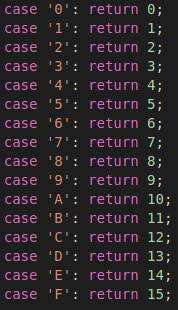
\includegraphics[height=8cm, width=3cm]{AA.png}}

Exemple:

\begin{center}
s={'A,/0'}

\textit{\textbf{Traitement(s,1)=Transfo(s[0])=11}}
\end{center}

\subsection{Cas récursif}

Pour déterminer le cas récursif, observons un exemple:

\begin{center}
\textbf{'A23' $\rightarrow$ 2595}
\end{center}

Imaginons que l$'$on découpe la chaine \textbf{'A23'} selon la définition 
récursive, on a

\begin{center}
\textbf{'A2 || 3' $\rightarrow$ 'A2' + 3 $*$ 1}    

$=$

\textbf{'A2 || 3' $\rightarrow$ 'A2' + 3}

(Le 3 après le $+$ est bien le nombre décimal et plus le caractère)
\end{center}

Et puis,

\begin{center}
\textbf{'A || 23' $\rightarrow$ 'A' + 2$*$16 + 3$*$1}

$=$

\textbf{'A || 23' $\rightarrow$ 'A' + 35}
\end{center}

On voit qu'il faut transformer le dernier caractère de la chaine et additioner le 
résultat de cette transformation au produit du facteur 16 (expliquation
dans le paragraphe suivant) avec le futur résultat du traitement de la chaine de 
caractères examptée du caractère déjà transformé.

La transformation citée depuis le début de ce rapport ne contient pas les
puissances de 16 permettant de passer effectivement d'un nombre hexadécimal à un
nombre décimal. En effet, cette transformation ne faisait qu'allusion à la
fonction \textit{convert(char hex)} préenregistrée pour nous. C'est pourquoi il 
est nécessaire de multiplier l'appel récursif par 16. 

De cette façon, les puissances seront toujours respectées étant donné que pour
atteindre le rang 2 (où nous avons donc 16\up{2}) il y a 2 appels récursifs
(et 1 appel de base). Nous aurons donc un facteur 16*16 au final pour ce rang, ce qui est correct.

I

\begin{center}
\textit{\textbf{Traitement(s, n) = Transfo(s[n-1]) + 16 * Traitement(s, n-1)}}
\end{center}


\subsection{Synthèse}


La formalisation récursive de \textit{Traitement} est donc:

\begin{center}

{\large si n = 0}

\textit{\textbf{Traitement(s, n) =}} 

\textit{\textbf{Transfo(s[0])}} 

\textit{\textbf{{\large ET}}} 

{\large sinon}

\textit{\textbf{Traitement(s, n) =}} 

\textit{\textbf{Traitement(s, n) = Transfo(s[n-1]) + 16 * Traitement(s, n-1)}} 

\end{center}


\section{Spécification}\label{specification}


Etant donné l'utilisation du Pseudo Langage vu au cours, il n'est pas nécessaire 
de vérifier que le pointeur représentant la chaine de caractères est valide
cependant nous allons vérifier que notre chaine existe grâce à sa longueur.

Notons que dans cette section nous reprendrons les notations introduite au début 
de ce rapport.

\begin{center}
{\large PréCondition} $\equiv n > 0$
\end{center}

L'objectif de notre fonction est de tranformer un nombre hexadécimale (sous forme 
de chaine de caractères) en un nombre décimale. En accord avec le code fourni, 
appelons la $hexa\_dec\_rec$. Elle prendra comme argument la chaine de caractère
donnée et sa longueur sous forme d$'$un entier.

\begin{center}
{\large Postondition} $\equiv hexa\_dec\_rec = Traitement(s,n)$
\end{center}

Au final l'interface de la fonnction est:

\begin{lstlisting}
/* 
 * @pre: n > 0
 * @post: hexa_dec_rec = Traitement(s,n)
 */
hexa_dec_rec(s,n)=(int x)
\end{lstlisting}


\section{Construction Récursive}\label{recur}

La structure générale d’une fonction/procédure récursive s’appuie sur une 
structure conditionnelle. On va donc remplir cette structure en trois étapes : 
(i) programmation défensive, (ii) cas de base, (iii) cas récursif(s).

\subsection{Programmation défensive}


En accord avec les préconditions, nous devons nous assurer que la chaine est
utilisable et donc que sa longueur n'est pas nulle. 

\begin{lstlisting}
hexa_dec_rec(s,n):
    if( n<=0 )
    then 
        r<-NULL;
\end{lstlisting}

Dans ce contexte de Pseudo-Langage théorique, je vérifie mes préconditions à 
l$'$aide d$'$une structure conditionnelle. Dans le code cette vérification est traduite par un \textit{assert} comme ceci:

\begin{lstlisting}
unsigned int hexa_dec_rec(char *hexa, int n){
  assert(hexa!=NULL && n>0);
\end{lstlisting}


\subsection{Cas de base}


Si la chaine de caractères n'en contient qu$'$un, on transforme directement ce 
caractère en son équivalent décimal.

\begin{lstlisting}
hexa_dec_rec(s,n):
    // {PréCondition}
    if (n = 1)
    then
        // {int x}
        r<-transfo(s[n-1];
        // {PostCondition}
\end{lstlisting}

\subsection{Cas récursif}


On suit la formulation récursive de \textit{Traitement}.

\begin{lstlisting}
else
    r<-Traitement(s, n) = Transfo(s[n-1]) + 16 * Traitement(s, n-1)
    // {PostCondition}
\end{lstlisting}


\subsection{Code récursif complet}


\begin{lstlisting}
hexa_dec_rec(s,n):
    if (n = 1)
    then
        r<-transfo(s[n-1];
    else
        r<-Traitement(s, n) = Transfo(s[n-1]) + 16 * Traitement(s, n-1)
\end{lstlisting}


\section{Traces d'exécution}\label{traces}


Dans cette section nous allons voire les valeurs qui sont stockées sur la pile
lors de l'exécution de notre fonction. Pour cela nous allons utiliser le même 
exemple que lors de la formalisation récursive de la fonction: $'$A23$'$.
\vspace{0.5cm}

\begin{center}
    

\begin{tabular}{|c|}
\\
\\
3\\
\hline
\textbf{1}
\end{tabular}~~
\begin{tabular}{|c|}
\\
2\\
3\\
\hline
\textbf{2}
\end{tabular}~~
\begin{tabular}{|c|}
10\\
32\\
3\\
\hline
\textbf{3}
\end{tabular}~~
\begin{tabular}{|c|}
2560\\
2\\
3\\
\hline
\textbf{4}
\end{tabular}~~
\begin{tabular}{|c|}
\\
2592\\
3\\
\hline
\textbf{5}
\end{tabular}~~
\begin{tabular}{|c|}
\\
\\
2595\\
\hline
\textbf{6}
\end{tabular}~~

\end{center}

Pour une facilité d'explication, se trouvent en dessous de chaque tableau représentant la pile le numéro lui correspondant.

\subsection{Descente récursive}



\subsubsection{Tableau 1}
Appel de la fonction. n > 1 donc on entre dans le cas récursif. Le résultat vaut
donc 3 qu'on empile.

\subsubsection{Tableau 2}
2ème appel de la fonction. n > 1 donc on entre dans le cas récursif. Le résultat 
vaut 2. qu'on empile.

\subsubsection{Tableau 3}
3ème appel de la fonction. n == 1donc on entre dans le cas de base. Le résultat 
vaut 10 qu'on empile.

\subsection{Remontée récursive}
Il est temps de faire les calculs.

\subsubsection{Tableau 4}
Etant donné qu'il y avait déjà eu 2 appels de la fonction lorsque le caractère
évalué nous rendait 10 comme résultat, nous devons multiplier ce résultat par 
16\up{2} ce qui donne 2560.

\subsubsection{Tableau 5}
N$'$oublions d$'$additionner à ça (2560) l$'$appel précédent qui rendait 2 comme
résultat mais avant lequel il y avait déjà eu 1 appel de la fonction. Il va donc 
de soi que nous devons multiplier 2 par 16\up{1} = 32 avant de faire l$'$addition.
(Multiplication avant addition car PEMDAS!). Nous avons donc maintenant une somme 
valant 2592.

\subsubsection{Tableau 6}
Cette fois, il nous faut additionner 2592 avec le premier appel de la fonction qui
renvoyait 3 comme résultat. Par définition, il n$'$y avait jamais eu d$'$appel de4
la fonction avant. Il est de ce fait inutile de chercher par quel facteur 3 doit 
être multiplié. Nous pouvons désormais faire notre dernière addition (2592 + 3), 
ce qui nous donne 2595 comme résultat final. 2595$_{10}$ équivaut bien à 
A23$_{16}$.


\section{Complexité}\label{complexite}


Nous allons, ici, nous charger de déterminer la complexité de notre fonction 
récursive. Pour cela nous allons éliminer la récurrence de proche en proche.

Le code de notre fonction étant:
\begin{lstlisting}
unsigned int hexa_dec_rec(char *hexa, int n){
  assert(hexa!=NULL && n>0);

  if(n==1)
    return convert(hexa[n-1]);
  else
    return convert(hexa[n-1]) + 16 * hexa_dec_rec(hexa, (n-1));
}//fin hexa\_dec\_rec()
\end{lstlisting}
\vspace{0.5cm}

Nous allons découper ce code en trois pour y voir plus clair:

\begin{center}
    a:
\end{center}
\begin{lstlisting}
  if(n==1)
    return convert(hexa[n-1]);
\end{lstlisting}

\begin{center}
    b:
\end{center}
\begin{lstlisting}
if(n==1)
    return convert(hexa[n-1]);
  else
    return convert(hexa[n-1]) + 16 * hexa_dec_rec(hexa, (n-1));
\end{lstlisting}

\begin{center}
    T(n-1):
\end{center}
\begin{lstlisting}
    return convert(hexa[n-1]) + 16 * hexa_dec_rec(hexa, (n-1));
\end{lstlisting}

Soit T(n), le coût d$'$un appel à hexa\_dec\_rec(hexa, (n)).
En ce qui concerne le cas de base, on va dire qu$'$il prend a opérations, a étant
constant. Pour ce qui est du cas récursif, on va dire qu$'$il demande b
opérations ainsi que le nombre d’opérations nécessaires par l’appel récursif,
c$'$est à dire T(n-1). Il vient le système suivant :

\begin{center}
T(n) = a si n=1
    
\textcolor{white}{----------------} = b+T(n-1) sinon
\end{center}

L’élimination de proche en proche consiste à réécrire plusieurs fois cette
équation en utilisant le cas récursif afin de faire apparaître un motif
reconnaissable.

\begin{center}
T(n) = b+T(n-1)
    
\textcolor{white}{----------} = b+b+T(n-2) 
    
\textcolor{white}{--------} = 3b+T(n-3) 

\textcolor{white}{--------} = 4b+T(n-4) 

\textcolor{white}{---} = ...\textcolor{white}{-------}
    
\textcolor{white}{-----------} = k$\times$b+T(n-k)

\end{center}

T (n-k) est une formulation tout à fait générale du temps d’exécution du Kème
appel récursif. On ne connait qu$'$une valeur particulière de T (.) : T (1) = 0.
On va donc essayer de faire apparaître cette valeur particulière. On a :

\begin{center}
n-k=1
    
\textcolor{white}{-----}-k=1-n    
    
\textcolor{white}{------}k=n-1
\end{center}

On insère cette valeur dans k $\times$ b + T (n-k), il vient :

\begin{center}
T (n) = (n-1) $\times$ b + T (1) = (n-1) $\times$ b + a $\in$
$\mathcal{O}(n)$
\end{center}



\section{Dérécursification}\label{derecur}


\subsection{Introduction du cas général}


Notre algorithme n'est pas de récursivité terminale et bien que la multiplication 
et l$'$addition soient chacune commutative et associative, la combinaison des 
deux ne l$'$est plus ( (5*3)+2 != 5*(3+2) ). Nous allons donc utiliser le cas
général de dérécursification vu au cours. Dans ce cas, nous allons simuler la pile
grâce à un TAD dont voici la sémantique:\vspace{0.5cm}

\noindent Type: 
    \begin{itemize}
        \item[$\bullet$] Stack
    \end{itemize}
    Utilise: 
    \begin{itemize}
        \item[$\bullet$] Boolean, Element
    \end{itemize}
    Opérations: 
    \begin{itemize}
        \item[$\bullet$] empty\_stack: $stack \rightarrow stack$
        \item[$\bullet$] is\_empty: $stack \rightarrow boolean$
        \item[$\bullet$] push: $stack \times element \rightarrow stack$
        \item[$\bullet$] pop: $stack \rightarrow stack$
        \item[$\bullet$] top: $stack \rightarrow element$
    \end{itemize}
    Précondtions:
    \begin{itemize}
        \item[$\bullet$] pop(s) is defined iff is\_empty(s) = False
        \item[$\bullet$] top(s) is defined iff is\_empty(s) = False
    \end{itemize}
    Axiomes: 
    \begin{itemize}
        \item[$\bullet$] is\_empty(empty\_stack) = True
        \item[$\bullet$] is\_empty(push(s, e)) = False
        \item[$\bullet$] pop(push(s, e)) = s
        \item[$\bullet$] top(push(s, e)) = e
    \end{itemize}

\subsection{Algorithme de transformation}

La conversion de la fonction récursive en itérative sera constituée d’une boucle
qui ne s’arrêtera que quand la Pile sera vide. Au début de chaque itération, on
dépile un contexte et on exécute les opérations en fonction de la valeur de pc. Ce
qui donne le code suivant :

\begin{lstlisting}
f (int x):
    // Il faut évidemment déclarer et initialiser une Pile vide.
    s <- empty_stack ();

    // On place sur la Pile le premier appel de la fonction, forcément, pc = 1 :
    s <- push(s, (x, 1));

    until is_empty(s) do
        // On dépile le premier contexte sur la pile
        (x, pc) <- top(s);
        s <- pop(s);

        // On choisit sur base de pc les opérations à effectuer:
        if (pc = 1)
            then
                if (cond(x))
                    then
                        r <- base(x);
                    else
                    /* Avant l appel récursif, on se souvient qu il faudra
                    continuer dans le bloc
                    */
                    s <- push(s, (x, 2))
                    // On empile ensuite l’appel récursif
                    s <- push(s, (progression(x), 1))
            else // pc = 2, donc
                // On récupère la dernière valeur de retour
                tmp <- r ;
                // On retourne le résultat calculé
                r <- operation(tmp , x);
end

// la variable r contient donc la valeur finale
\end{lstlisting}

On considère que pc = 1 quand on entre dans la fonction et pc = 2 au retour de
l’appel récursif.


\subsection{Transformation du code}

\begin{center}
    Code récursif:
\end{center}
\begin{lstlisting}
hexa_dec_rec(s,n):
    if (n = 1)
    then
        r<-transfo(s[n-1];
    else
        r<-Traitement(s, n) = Transfo(s[n-1]) + 16 * Traitement(s, n-1)
\end{lstlisting}

\begin{center}
    Code récursif générique:
\end{center}
\begin{lstlisting}
f(s,n):
    if (cond(n))
    then
        r<-g(s);
    else
        r<-G(s, f(s,n);
\end{lstlisting}

\begin{center}
    Code itératif générique:
\end{center}
\begin{lstlisting}
f_derec(s, n):
    p <- empty_stack();
    a <- 0;
    b <- s;
    until cond(a) do
        p <- push(p, b[a]);
        a <- h(a);
    end
    until is_empty(p) do
        b <- top(p);
        p <- pop(p);
        r <- G(s, r);
    end
\end{lstlisting}

\begin{center}
    Code itératif final:
\end{center}
\begin{lstlisting}
hexa_dec_rec_derec(s, n):
    p <- empty_stack();
    a <- 0;
    b <- s;
    until a = n do
        p <- push(p, b[a]);
        a <- a+1;
    end
    until is_empty(p) do
        b <- top(p);
        p <- pop(p);
        r <- transfo(b) + 16 * r ;
    end
\end{lstlisting}




\end{document}
